\subsection{Hydraulic properties}
\label{sec:h_properties}

Recalling the balance equations for fluid mass (\ref{eqn:mass_pormed_deform}) and fluid momentum (\ref{eqn:momentum_balance_fluid}), i.e. Darcy's law the following material quantities needs to be specified: fluid densities $\rho^\Phase$, fluid viscosities $\mu^\Phase$, permeabilities $\PermRelP^{\gamma}, \PermTensor$, and porosity $n$.
Fluid phase pressures $p^\Phase$, saturations $S^\Phase$ and velocities $\VelocityVector^{\Phase s}$ are considered state variables.

%-------------------------------------------------------------------------
\subsubsection{Density - $\rho$}

Density is considered as a mechanical material property (sec. \ref{sec:m_properties}).

%-------------------------------------------------------------------------
\subsubsection{Viscosity - $\Viscosity^\Phase$}

Viscosity is defined as shearing stress per unit area divided by a
velocity gradient and it has the dimension of $N\,s/m^2$ or
$Pa\,s$.

\begin{figure}[htb!]
\begin{center}
\footnotesize
\includegraphics[width=0.75\columnwidth]{chapter20/figures/visco9.eps}
\caption{Water viscosity as a function of temperature}
\label{fig:visco9}
\end{center}
\end{figure}

\begin{itemize}
%.........................................................................
 \item
Non-isothermal flow of water (de Marsily 1986) (Fig. \ref{fig:visco9})
\begin{eqnarray}
\Viscosity^w (\Temperature)
=
2.285 \times 10^{-5}
+
1.01 \times 10^{-3} \log\Temperature
\end{eqnarray}
%.........................................................................
\item
Non-isothermal flow of gas (Reid et al. 1988)
(Fig. \ref{fig:visco7})
\begin{eqnarray}
\Viscosity^g (\Pressure,\Temperature)
=
\Viscosity_0
\left(
1 + \frac{A\Pressure_r^{3/2}}{B\Pressure_r+(1+C\Pressure_r^D)^{-1}}
\right)
\end{eqnarray}
%
with the following parameters:
\begin{eqnarray}
\begin{array}{ll}
\Pressure_r = \Pressure / \Pressure_{\mbox{\footnotesize crit}}
&
\Temperature_r = \Temperature / \Temperature_{\mbox{\footnotesize crit}}
\\
A = \D\frac{\alpha_1}{T_r} \exp (\alpha_2 T_r^a)
&
B = A(\beta_1 T_r - \beta_2)
\\
C = \D\frac{\gamma_1}{T_r} \exp (\gamma_2 T_r^c)
&
D = \D\frac{\delta_1}{T_r} \exp (\delta_2 T_r^d)
\end{array}
\\
\begin{array}{lll}
\Pressure_{\mbox{\footnotesize crit}} = 33.9 \times 10^4 \, Pa
&
\Temperature_{\mbox{\footnotesize crit}} = 126.2 \, K
\\
\alpha_1 = 1.9824\times 10^{-3}  &  \alpha_2 = 5.2683  &  a = -0.5767 \\
\beta_1  = 1.65552               &  \beta_2  = 1.2760  &  \\
\gamma_1 = 0.1319                &  \gamma_2 = 3.7035  &  c = -79.8678 \\
\delta_1 = 2.9496                &  \delta_2 = 2.9190  &  d = -16.6169
\end{array}
\nonumber
\end{eqnarray}

\begin{figure}[htb!]
\begin{center}
\footnotesize
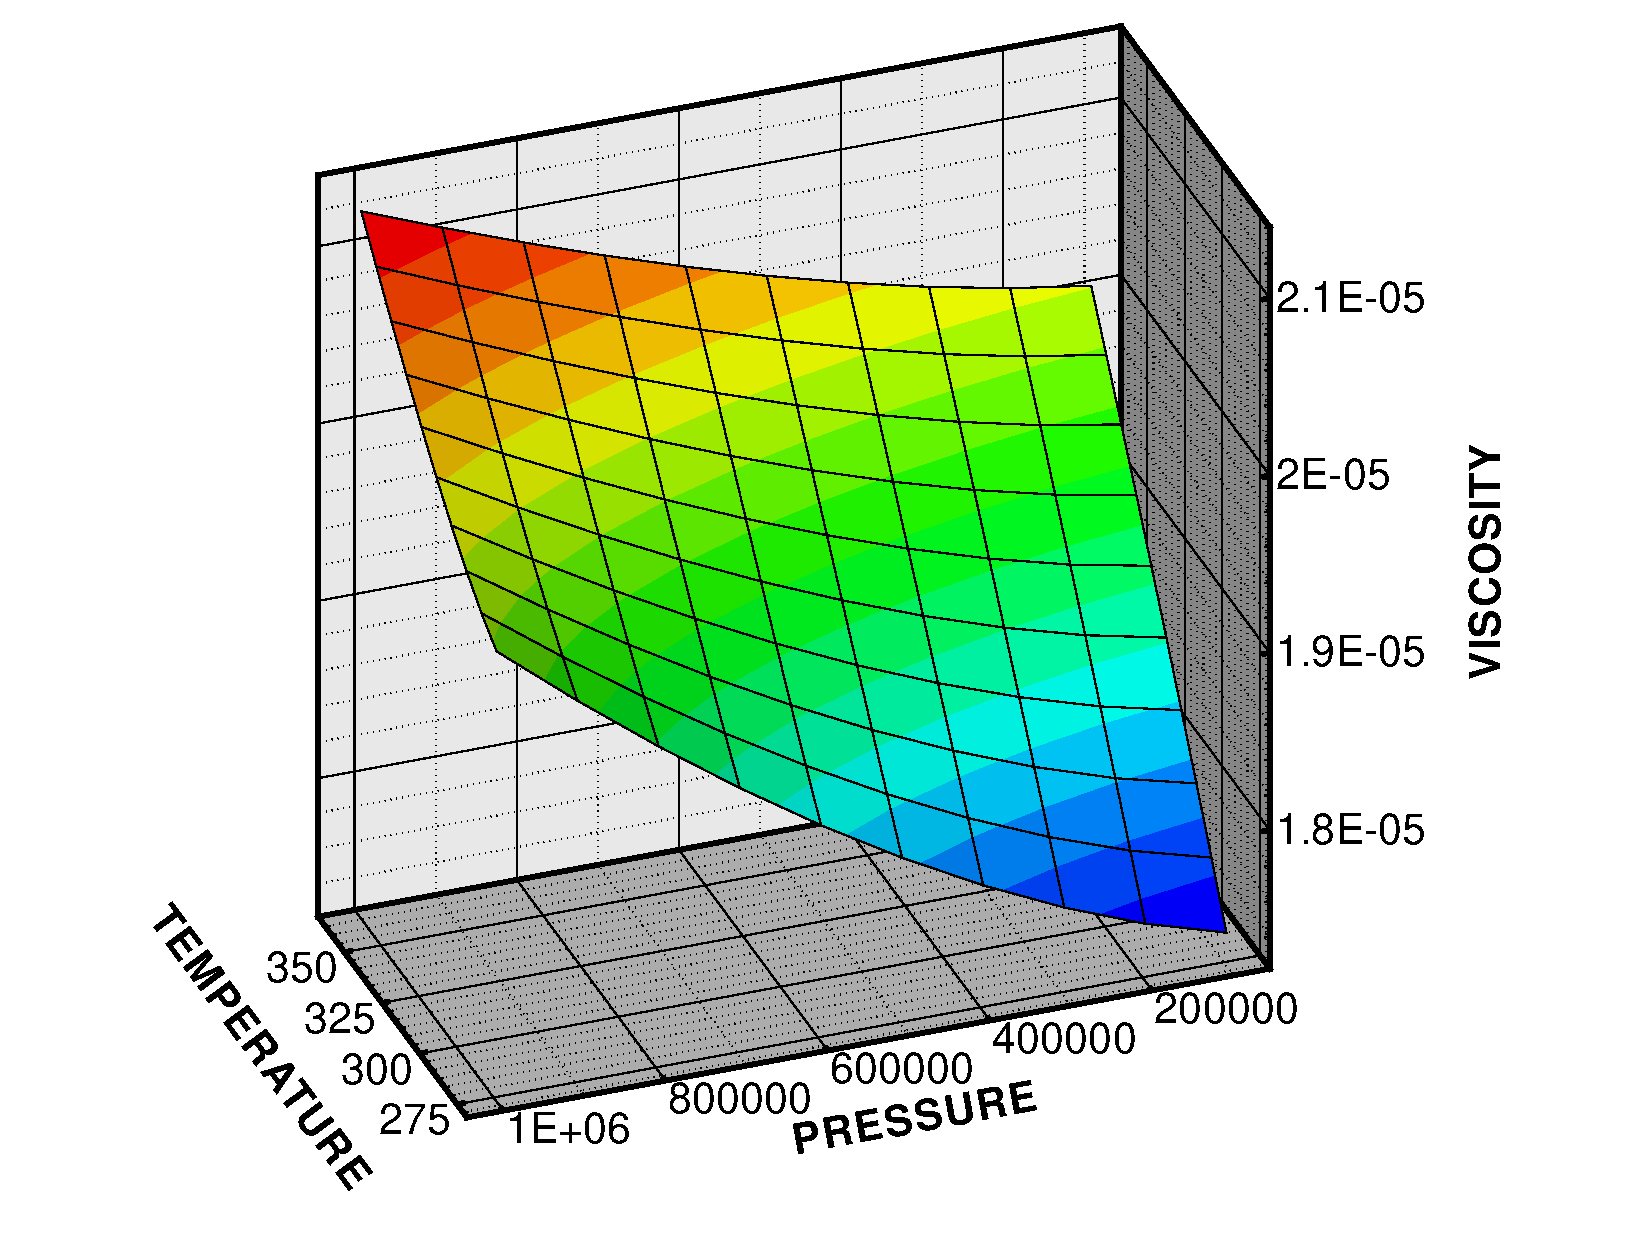
\includegraphics[width=0.6\columnwidth]{chapter20/figures/viscosity.eps}  % Filename.eps
\caption{Gas viscosity as a function of temperature and pressure}
\label{fig:visco7}
\end{center}
\end{figure}
%

\item
Non-isothermal flow of brines
(Lever and Jackson 1985)
\begin{eqnarray}
\Viscosity^w (\Temperature,\Conc)
=
\Viscosity_0
\frac{1+1.85\omega-4.1\omega^2+44.5\omega^3}{1+0.7063\zeta-0.04832\zeta^2}
\end{eqnarray}
with:
\begin{eqnarray}
\omega = \frac{\Conc}{\Density}
\quad , \quad
\zeta = \frac{T-150�C}{100�C}
\end{eqnarray}

\end{itemize}


%-------------------------------------------------------------------
\subsubsection*{Relative permeability - $\PermRelP^\Phase(\Saturation^\Phase)$}

For porous media containing more than one fluid, the concept of
relative permeability is introduced.  The relative permeability is
used to calculate the effective permeability
$(\PermRelP^\Phase\Saturation^\Phase)\PermTensor$, which is
described in the extended Darcy law.  The relationship depends
strongly on the saturations. Different relationships are possible:
constant values, user-defined functions, linear functions,
potential functions, or functions found in literature, such as the
van Genuchten Model (1980)
\begin{eqnarray}
\PermRelS(\Saturation^l)
=
\SaturationEff^{1/2}
\left(
1-(1-\SaturationEff^{1/\beta})^\beta
\right)^2
\label{eqn:relative_permeability_saturation}
\end{eqnarray}

$\PermTensor$ is the permeability of fully liquid saturated porous medium, i.e. the maximum permeability for liquid flow.
%
Capillary pressure and relative permeabilities are among
the most important parameters affecting multi-phase flow.

\begin{figure}[htb!]
\begin{center}
\footnotesize
\includegraphics[width=0.49\columnwidth]{chapter20/figures/persat.eps}  % Filename.eps
\includegraphics[width=0.49\columnwidth]{chapter20/figures/capsat.eps}  % Filename.eps
\caption{Relative permeability (left) and capillary pressure (right) as functions of liquid saturation for two different porous media: crystalline rock and bentonite}
\label{fig:capillarity}
\end{center}
\end{figure}

%-------------------------------------------------------------------
\subsubsection*{Capillary pressure - $\CapillaryPressure(\Saturation)$}

The capillary pressure can be defined as the tendency of a porous
medium to suck in the wetting fluid phase or to repel the
non-wetting phase.  Capillary pressure results from the pressure
discontinuity at the interface between two immiscible fluids.
Capillary pressure depends on the geometry of the void space, on
the nature of solids and liquids and on the degree of saturation.
In porous media the geometry of the void space is idealized. Thus,
the dependence reduces to saturation for any given porous media.
Care has to be taken, as capillary pressure is not the same for
drainage and re-wetting. The function connecting capillary
pressure and saturation has to be determined by laboratory
experiments for every new porous medium.
Frequently, an analytical
functions is used, such as the van Genuchten (1980) model
%
\begin{eqnarray}
\CapillaryPressure(\Saturation^l)
=
\left\{
\begin{array}{ll}
0 & \Saturation^l > \SaturationMax^l
\\
\frac{\Density^l g}{\alpha} (\SaturationEff^{-1/m}-1)^{1/n} &
\SaturationRes^l < \Saturation^l < \SaturationMax^l
\\
\CapillaryPressureMax & \Saturation^l < \SaturationRes^l
\end{array}
\right.
\label{eqn:capillary_pressure_saturation}
\end{eqnarray}

whit the effective saturation
\begin{eqnarray}
\SaturationEff
=
\frac{\Saturation^l - \SaturationRes^l}{1-\SaturationRes^l}
=
\left( 1 + (\alpha \, \CapillaryPressure)^n \right)^m
\qquad , \qquad \CapillaryPressure > 0
\end{eqnarray}


